\documentclass[notes,11pt, aspectratio=169]{beamer}

\usepackage{pgfpages}
% These slides also contain speaker notes. You can print just the slides,
% just the notes, or both, depending on the setting below. Comment out the want
% you want.
\setbeameroption{hide notes} % Only slide
%\setbeameroption{show only notes} % Only notes
%\setbeameroption{show notes on second screen=right} % Both

\usepackage{helvet}
\usepackage[default]{lato}
\usepackage{array}

\usepackage{caption}
\usepackage{subcaption}

\usepackage{tikz}
\usepackage{verbatim}
\setbeamertemplate{note page}{\pagecolor{yellow!5}\insertnote}
\usetikzlibrary{positioning}
\usetikzlibrary{calc}
\usetikzlibrary{arrows}
\usetikzlibrary{decorations.markings}
\usetikzlibrary{shapes.misc}
\usetikzlibrary{matrix,shapes,arrows,fit,tikzmark}
\usepackage{amsmath}
\usepackage{mathpazo}
\usepackage{lipsum}
\usepackage{amsmath, amsfonts, amssymb}
\usepackage{multimedia}
\usepackage{graphicx}
\usepackage{multirow}
\usepackage{graphicx}
\usepackage{dcolumn}
\usepackage{bbm}
\newcolumntype{d}[0]{D{.}{.}{5}}

\usepackage{changepage}
\usepackage{appendixnumberbeamer}
\newcommand{\beginbackup}{
   \newcounter{framenumbervorappendix}
   \setcounter{framenumbervorappendix}{\value{framenumber}}
   \setbeamertemplate{footline}
   {
     \leavevmode%
     \hline
     box{%
       \begin{beamercolorbox}[wd=\paperwidth,ht=2.25ex,dp=1ex,right]{footlinecolor}%
%         \insertframenumber  \hspace*{2ex} 
       \end{beamercolorbox}}%
     \vskip0pt%
   }
 }
\newcommand{\backupend}{
   \addtocounter{framenumbervorappendix}{-\value{framenumber}}
   \addtocounter{framenumber}{\value{framenumbervorappendix}} 
}


\usepackage{graphicx}
\usepackage[space]{grffile}
\usepackage{booktabs}

\DeclareUnicodeCharacter{0301}{\'{e}}
\DeclareUnicodeCharacter{0303}{}

% These are my colors -- there are many like them, but these ones are mine.
\definecolor{blue}{RGB}{0,114,178}
\definecolor{red}{RGB}{213,94,0}
\definecolor{yellow}{RGB}{240,228,66}
\definecolor{green}{RGB}{0,158,115}




%% I use a beige off white for my background
\definecolor{MyBackground}{RGB}{255,253,218}

%% Uncomment this if you want to change the background color to something else
%\setbeamercolor{background canvas}{bg=MyBackground}

%% Change the bg color to adjust your transition slide background color!
\newenvironment{transitionframe}{
  \setbeamercolor{background canvas}{bg=yellow}
  \begin{frame}}{
    \end{frame}
}

\setbeamercolor{frametitle}{fg=blue}
\setbeamercolor{title}{fg=black}
\setbeamertemplate{footline}[frame number]
\setbeamertemplate{navigation symbols}{} 
\setbeamertemplate{itemize items}{-}
\setbeamercolor{itemize item}{fg=blue}
\setbeamercolor{itemize subitem}{fg=blue}
\setbeamercolor{enumerate item}{fg=blue}
\setbeamercolor{enumerate subitem}{fg=blue}
\setbeamercolor{button}{bg=MyBackground,fg=blue,}



% If you like road maps, rather than having clutter at the top, have a roadmap show up at the end of each section 
% (and after your introduction)
% Uncomment this is if you want the roadmap!
 \AtBeginSection[]
 {
    \begin{frame}
        \frametitle{Roadmap of Talk}
        \tableofcontents[currentsection]
    \end{frame}
 }
\setbeamercolor{section in toc}{fg=blue}
\setbeamercolor{subsection in toc}{fg=red}
\setbeamersize{text margin left=30pt,text margin right=30pt} 

\newenvironment{wideitemize}{\itemize\addtolength{\itemsep}{10pt}}{\enditemize}

\usepackage{environ}
\NewEnviron{videoframe}[1]{
  \begin{frame}
    \vspace{-8pt}
    \begin{columns}[onlytextwidth, T] % align columns
      \begin{column}{.58\textwidth}
        \begin{minipage}[t][\textheight][t]
          {\dimexpr\textwidth}
          \vspace{8pt}
          \hspace{4pt} {\Large \sc \textcolor{blue}{#1}}
          \vspace{8pt}
          
          \BODY
        \end{minipage}
      \end{column}%
      \hfill%
      \begin{column}{.42\textwidth}
        \colorbox{green!20}{\begin{minipage}[t][1.2\textheight][t]
            {\dimexpr\textwidth}
            Face goes here
          \end{minipage}}
      \end{column}%
    \end{columns}
  \end{frame}
}

\title[]{\textcolor{blue}{Causal Inference with Synthetic Controls:\\ Estimating the Economic Costs of Conflict }}
%\author[PGP]{}
\institute[GSB]{\small{\begin{tabular}{c}
Alexander J. Almeida \\
Stanford Graduate School of Business\\
\end{tabular}}}

\date{November 17, 2022}

\usepackage[backend=biber,style=apa]{biblatex}
\addbibresource{ref.bib}

%\usepackage{hyperref}
\hypersetup{
  colorlinks=false,
  linkcolor=, 
  urlcolor=
}


\makeatletter
\newcommand\disablecolorlinks{\def\HyColor@UseColor##1{}}
\makeatletter
\addtobeamertemplate{headline}{\disablecolorlinks{}}{}

\begin{document}

%%% TIKZ STUFF
\tikzset{   
        every picture/.style={remember picture,baseline},
        every node/.style={anchor=base,align=center,outer sep=1.5pt},
        every path/.style={thick},
        }
\newcommand\marktopleft[1]{%
    \tikz[overlay,remember picture] 
        \node (marker-#1-a) at (-.3em,.3em) {};%
}
\newcommand\markbottomright[2]{%
    \tikz[overlay,remember picture] 
        \node (marker-#1-b) at (0em,0em) {};%
}
\tikzstyle{every picture}+=[remember picture] 
\tikzstyle{mybox} =[draw=black, very thick, rectangle, inner sep=10pt, inner ysep=20pt]
\tikzstyle{fancytitle} =[draw=black,fill=red, text=white]
%%%% END TIKZ STUFF

% Title Slide
\begin{frame}
\maketitle
 % \centering The views expressed do not necessarily reflect the position of the Federal Reserve Bank of New York or the Federal Reserve System.
\end{frame}



%%% OUTLINE %%%

% Motivation: Setting in Spain
%   1. Show the map 
%   2. Talk about Basque independence movement and terrorism
%   3. Talk about ETA terrorism and show the timeline of deaths. 
%       a. Emphasize the severity is a measure of treatment 
%       b. Emphasize that treatment was localized inside of the Basque region
%   4. As social scientists, we might wonder how the conflict impacted material
%       well-being. A well-worn proxy is GDP. Then we want to look at the impact
%       of the conflict on macroeconomic aggregates. However, there is lots of 
%       confounding. How do we proceed? 
% 
% Problem statement: The Main Question
%   1. First pass: we could just compare the means before and after the terrorism. 
%       by extension we could look at the evolution of gdp per capita to get see the effect. 
%       - Failure: Spain as a country suffered a macroeconomic downturn in the ???, 
%           so saying something causal from mean comparison is not possible.

% Introduce the method: 
%   1. Quote from the Athey/Imbens paper
%   2. The Synthetic Control constructed in Abadie and Gardeazabal 2003
        % The math!
%   3. Sell the method
%       a. 
% Show some results
% ? Discuss the other exercise in the paper 
% Zoom out: Discuss some of the other settings where synthetic controls have been used. 
%   Briefly walk through those together
%   - Abadie Diamond Hainmueller (2015) German reunification
%   - Focus in on the Abadie, Diamond, and Hainmueller paper
% Demo the R packages and show some results
%   - Package names and citations. Note the fact that many are pretty new.
%       - tidysynth (Dunford at Georgetown)
%       - gsynth (Yiqing Xu and Licheng Liu)
%       - synth (original authors)
%       - sc tools? Has some more tools
%       - scpi: Cattaneo et. al is uncertainty quantification for sc methods

% TODO
% 1. Return back to the applications section if time permits

% Section 0: Introduction
\begin{frame}{}
    \begin{figure}
    \centering
        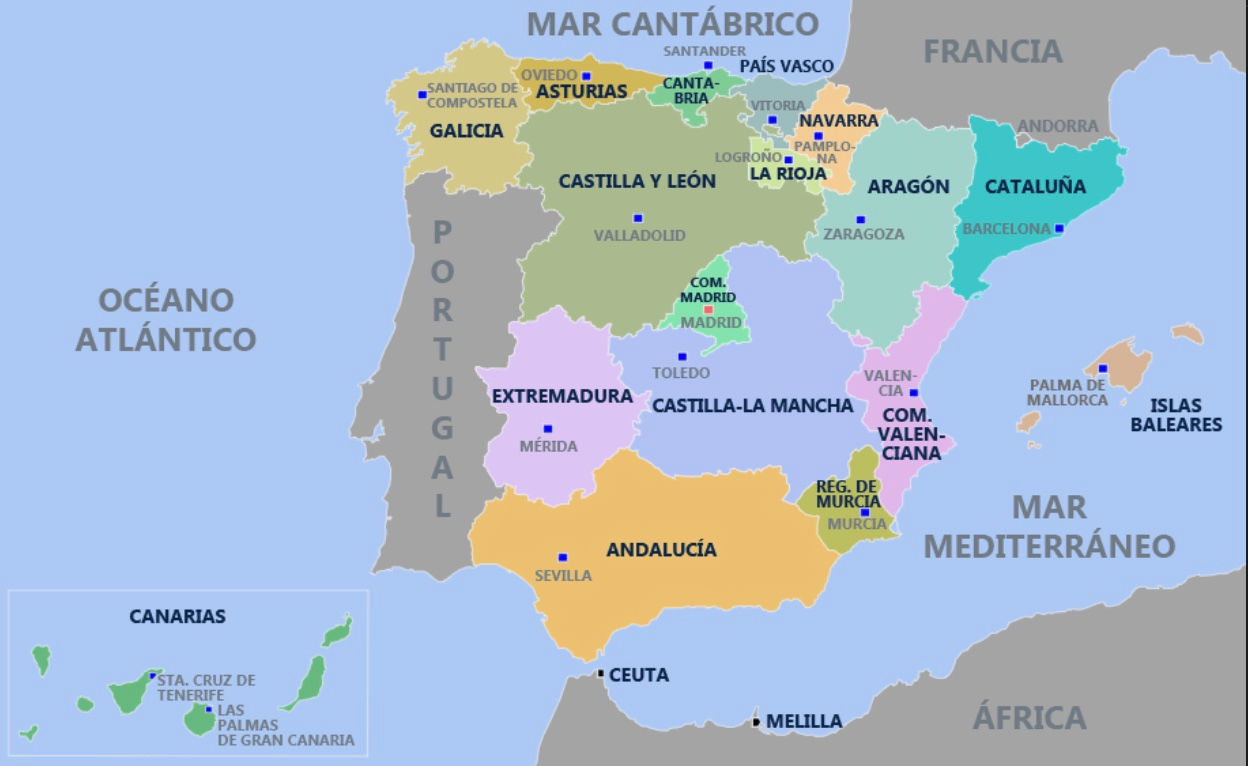
\includegraphics[width = .7\linewidth]{figures/mapa.png}
        \label{fig:map}
    \end{figure}
\end{frame}

\begin{frame}{}
    \begin{wideitemize}
        \item Spain is organized into 17 "autonomous communities" 
        \item Each community holds a large degree of government power \medskip 
        \begin{wideitemize}
            \item Greater power still deferred to "historical nationalities": Galicia, Basque Country, Catalonia
        \end{wideitemize}
        \item Catalonia and the Basque Country have seen major separatist movements 
    \end{wideitemize}
\end{frame}

\begin{frame}{}
    \begin{figure}
    \centering
        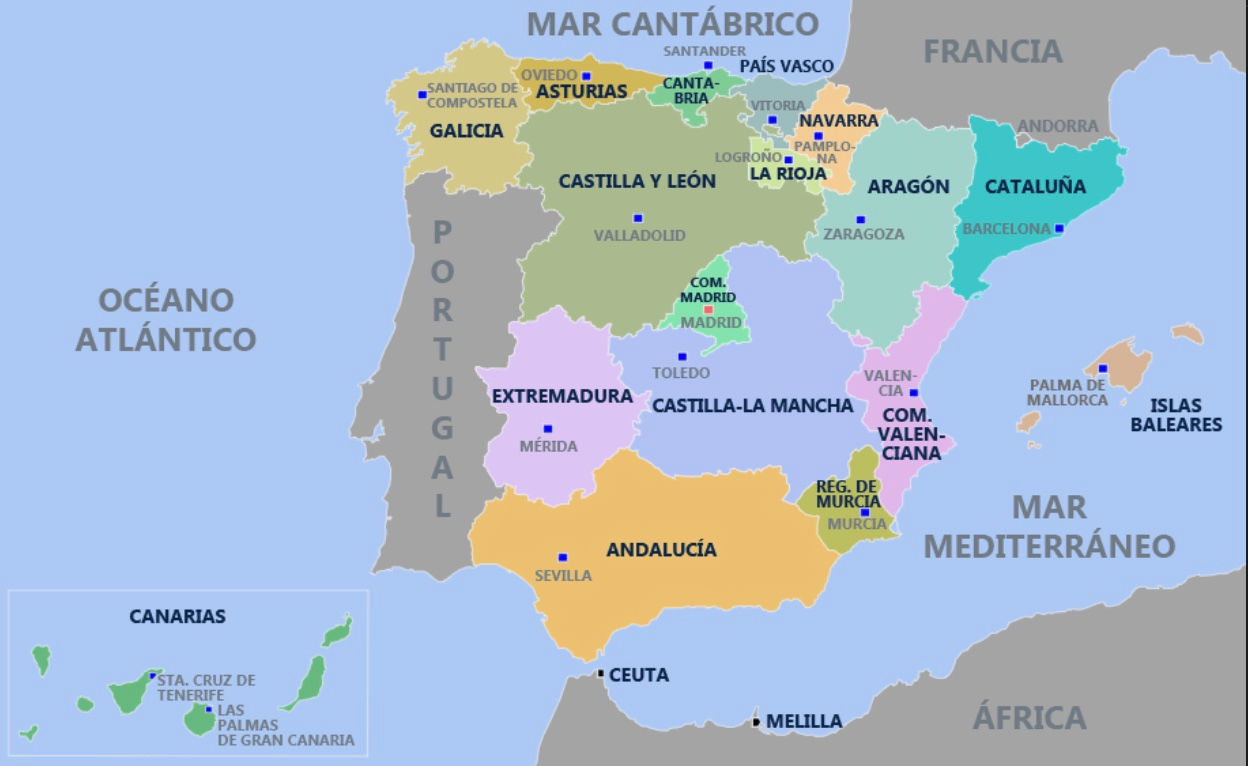
\includegraphics[width = .7\linewidth]{figures/mapa.png}
        \label{fig:map2}
    \end{figure}
\end{frame}

\begin{frame}
    \begin{wideitemize}
        \item Euskadi Ta Askatasuna (ETA) formed to support Basque separatism
        \item Beginning in 1960s, begin terrorist activities
    \end{wideitemize}
\end{frame}

\begin{frame}
    \begin{figure}
        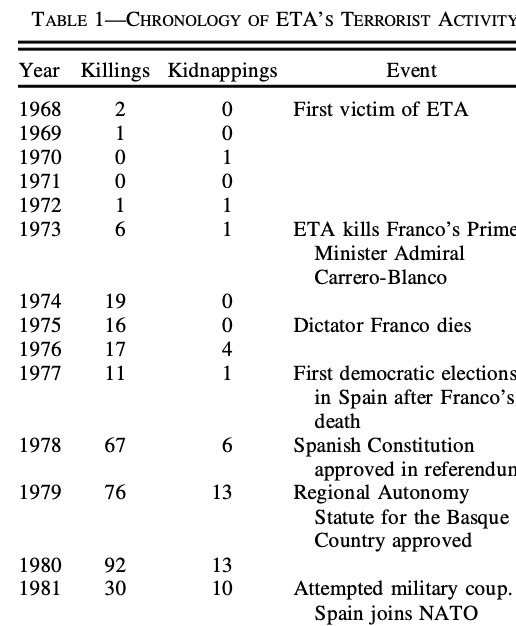
\includegraphics[width = .4\linewidth]{figures/tab11.png}
    \end{figure}
\end{frame}

\begin{frame}
    \begin{figure}
        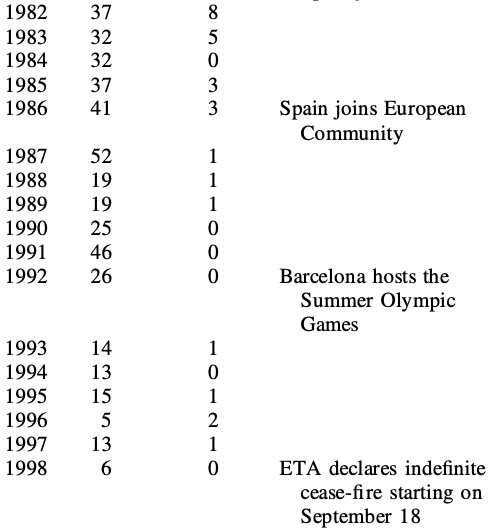
\includegraphics[width = .4\linewidth]{figures/tab12.png}
    \end{figure}
\end{frame}

\begin{frame}{}
    \begin{wideitemize}
        \item Question: What was the impact of terrorism on the people of the Basque Region? \pause 
        \item Less ambitious
        \begin{wideitemize} 
            \item What was the \textbf{economic} impact of terrorism on the people of the Basque Region? 
            \item Can we quantify this effect?
        \end{wideitemize}
    \end{wideitemize}
\end{frame}

\section{Empirical considerations}

\begin{frame}{Empirical considerations}
    A few stylized facts: \medskip 
    \begin{wideitemize}
        \item Terrorist activities took place in Basque country at a higher frequency than rest of Spain \medskip 
        \begin{wideitemize}
            \item Deaths per 1 million inhabitants per year: 8.17 Basque Country, 0.22 Rest of Spain (1968-1997) \pause
        \end{wideitemize}
        \item The Basque conflict had "no direct economic motivation" (\cite{abadie_economic_2003}, pp. 114) \pause 
        \item The Basque region experienced less growth than other Spanish regions
    \end{wideitemize}
\end{frame}

\begin{frame}{Empirical considerations}
    \begin{figure}
    \centering
        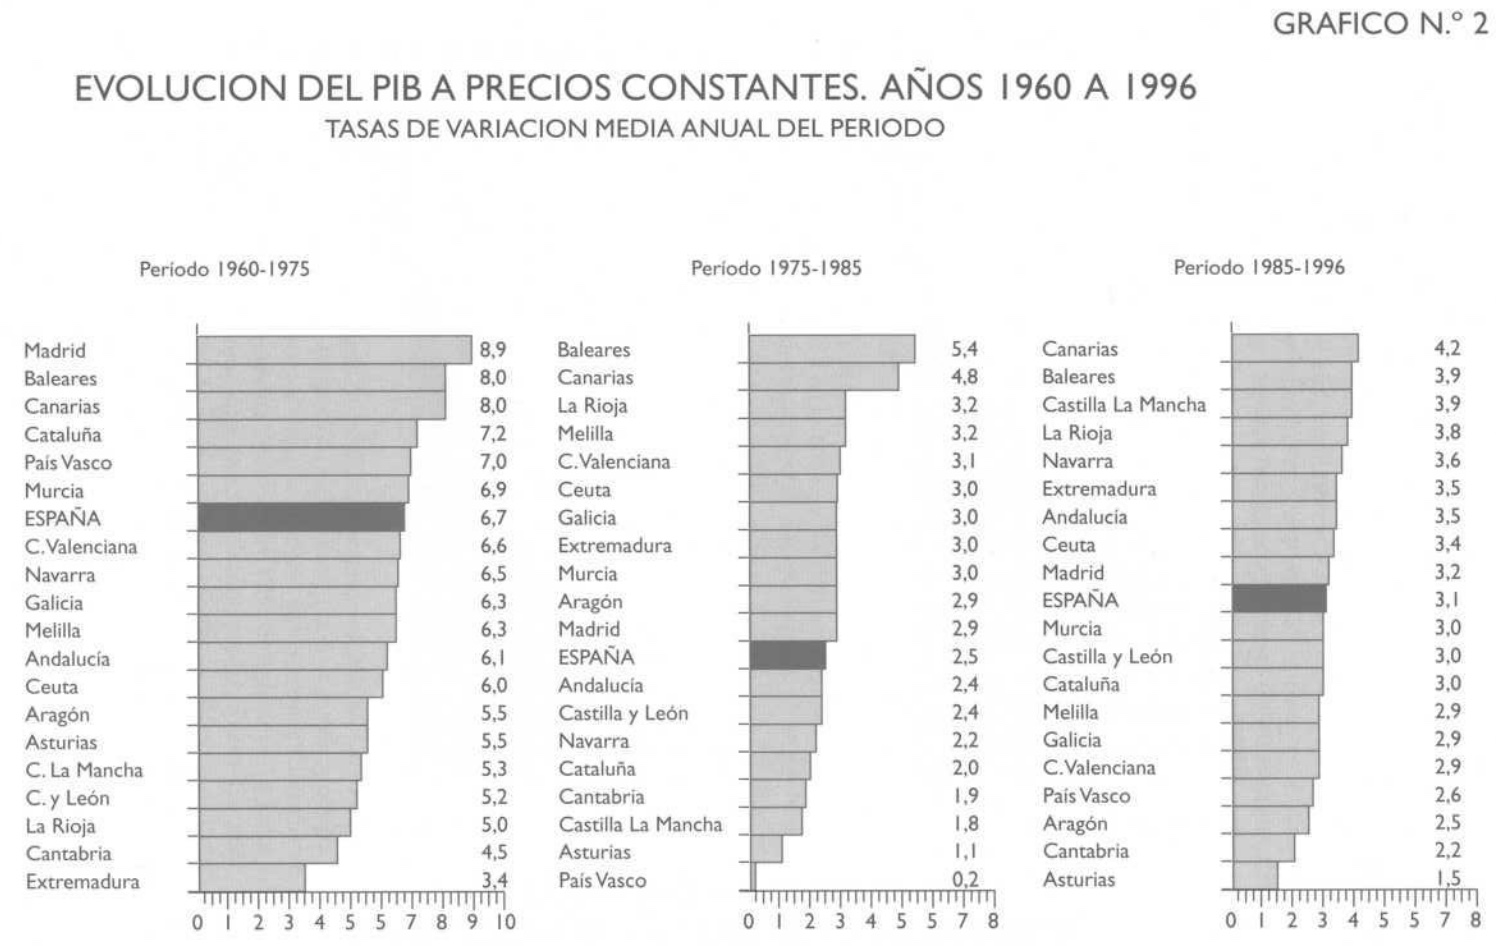
\includegraphics[width = .75\linewidth]{figures/evolucion_pib.png}
        \label{fig:evolucion}
        \caption*{\small Source: \cite{fundacion_bbv_renta_1999}}
    \end{figure}
\end{frame}

\begin{frame}{Empirical considerations}
    How do we quantify the effect of terrorism? \bigskip
    \begin{wideitemize}
        \item A na\"ive comparison of means before and after terrorism \medskip 
        \begin{wideitemize} 
            \item ignores time-varying dynamics that are independent of terrorism 
            \item e.g. Business cycle variations in macroeconomic aggregates
        \end{wideitemize}
        \item Comparing Basque country to other regions of Spain \medskip 
            \begin{wideitemize}
                \item Concentration of terrorism in Basque country supports this method
            \end{wideitemize}
    \end{wideitemize}    
\end{frame}

\begin{frame}{Empirical considerations}
    How do we quantify the effect of terrorism? \pause \\
    \bigskip 
    
    \rightline{Compare the outcomes of Basque country to other regions that are similar.}
    \rightline{\textcolor{purple}{Issue: we can't just compare it to the rest of Spain.}}   
\end{frame}

\begin{frame}{Empirical considerations}
    \begin{figure}
        \centering
        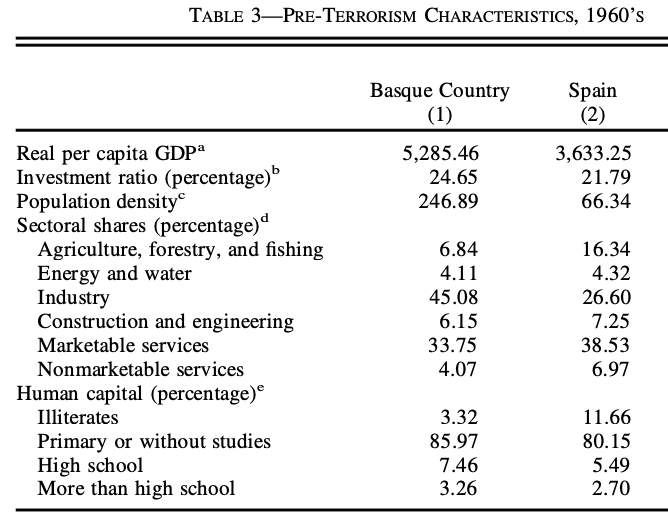
\includegraphics[width = .6\textwidth]{figures/balance panel.png}
        \label{fig:balance}
    \end{figure}
\end{frame}

\begin{frame}{Empirical considerations}
    How do we quantify the effect of terrorism? \\
    \bigskip 
    
    \rightline{Compare the outcomes of Basque country to other regions that \textbf{are similar}.} \pause 

    \bigskip \bigskip 
    
    Any experimental control group of this form will be a weighted average of the options available. \medskip
        \begin{wideitemize}
           \item Comparing to rest of spain gives equal weights 
           \item A difference-in-differences approach would set the weight to 1 for the control regions of interest
           \item We can choose the weights more carefully: \textbf{synthetic control}
        \end{wideitemize}
    
\end{frame}

\begin{frame}{Empirical considerations}
    \begin{figure}
        \centering
        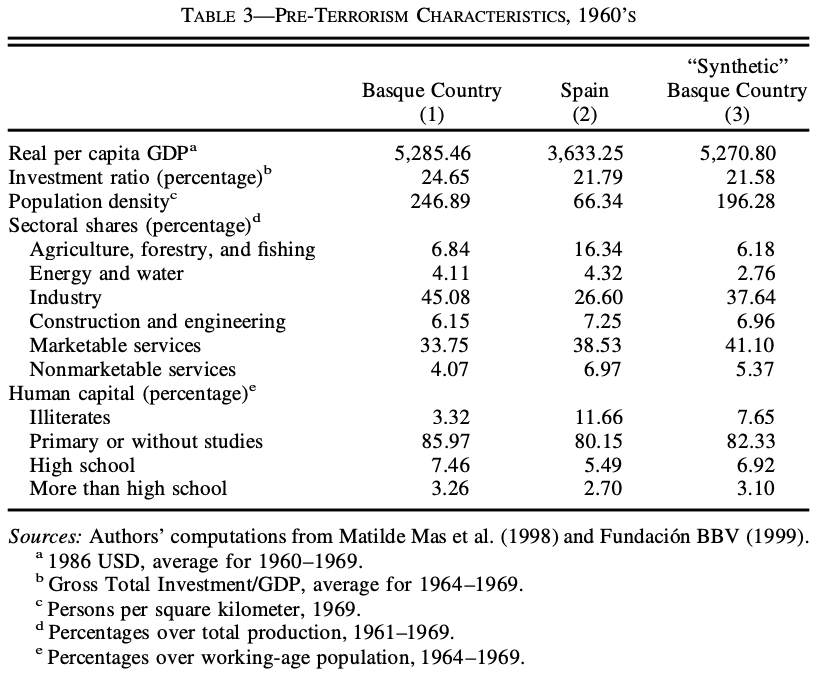
\includegraphics[width = .6\textwidth]{figures/balance panel all.png}
        \label{fig:balance_all-2}
    \end{figure}
\end{frame}

\section{Methods}

\begin{frame}{Methods}
\center "The synthetic control approach developed by \cite{abadie_synthetic_2010} and \cite{abadie_economic_2003} is \textit{arguably the most important innovation} in the policy evaluation literature in the last 15 years." 
	\\ \medskip \medskip \medskip \hspace*{\fill} --\cite{athey_state_2017}
\end{frame}

\begin{frame}{Methods}
    \begin{wideitemize}
        \item Suppose there are $J$ potential control regions. \pause 
        \item Let $W = (w_1, \ldots, w_J)' \in \mathbb R^J$ be the weights. Each $W$ corresponds to 
        a different synthetic control region. \pause 
        \item Goal: Choose $W$ such that the synthetic control region resembles the actual region. \pause \medskip
        \begin{wideitemize}
            \item Let $X_1 \in \mathbb R^K$ be the vector of pre-treatment observables. 
            \item Let $X_0 \in \mathbb R^{K \times J}$ be the matrix of pre-treatment observables for all regions. 
            \item We want to minimize $\| X_1 - X_0 W\|$
        \end{wideitemize}
    \end{wideitemize}
\end{frame}

\begin{frame}{Methods}
    \begin{itemize}
        \item We want minimize something like the residual sum of squares \pause 
        \item Operationalize this by letting $V \in \mathbb R^{K \times K}$ be diagonal (more generally, positive semi-definite, see \cite{abadie_synthetic_2010}). For each $k \in K$, $V_{kk}$ represents the relative weight that we give to the observable pre-treatment variable indexed by $k$. \pause 
        \item Define the norm: 
        \[\|X_1 - X_0 W\| := (X_1 - X_0 W)' V (X_1 - X_0W)\] \pause  
        \item We can but don't need to impose some constraints on the weights as well
        \begin{itemize}
            \item (W1) $\forall j$, $w_j \in [0,1]$ \quad \quad  (No extrapolation - convex hull)
            \item (W2) $w_1 + w_2 + \cdots + w_J = 1$
        \end{itemize}
        \item What should we choose for $V$? 
    \end{itemize}
\end{frame}

\begin{frame}{Methods}
    \begin{wideitemize}
        \item In principle, $V$ is the relative importance of pre-treatment observables. 
        \item We may have some priors based on prior literature \medskip
        \begin{wideitemize}
            \item E.g. we are using macroeconomic variables advanced by \cite{barro_economic_2004}. 
        \end{wideitemize}
    \end{wideitemize}    
\end{frame}

\begin{frame}{Methods}
     
        We may also take the "eclectic approach" advanced in this paper. \pause 
    
    \begin{itemize}
    
            \item Let $\mathcal W$ denote the subset of $\mathbb R^J$ satisfying (W1) and (W2). \pause 
            
            \item We have discussed choosing weights to minimize the weighted sum of squared errors, which is conditional on $V$,
            \[ W^*(V) = \text{argmin}_{W \in \mathcal W} (X_1 - X_0 W)' V (X_1 - X_0 W) \] \pause 
            
            \item Let $Z_1 \in \mathbb R^{10}$ be the per capita gdp in Basque Country for the ten years prior to intervention. 
            
            \item Let $Z_0 \in \mathbb R^{10\times J}$ be the same, but for the potential control regions. \pause 
            
            \item Now choose $V$ to minimize the sum of squared error between the true values $Z_1$ and the synthetic region's values $Z_0 W^*(V)$. 
            \[ V^* = \text{argmin}_{V \in \mathcal V} (Z_1 - Z_0 W^*(V) )' (Z_1 - Z_0 W^*(V) ) \]
            where $\mathcal V$ is the set of all diagonal (positive semi-definite) matrices over $\mathbb R$. 
        
    \end{itemize}    
    
\end{frame}

\begin{frame}{Methods}
    Performing this method tells us that 
    \[\texttt{Basque} = 0.8508(\texttt{Catalonia}) + 0.1492 (\texttt{Madrid})\]

    Based on the construction, we expect that  \medskip 
    \begin{wideitemize}
        \item pre-intervention observables of Basque region and synthetic Basque region are close, and
        \item pre-intervention per capita GDP time series for Basque and synthetic Basque regiones are close
    \end{wideitemize}
\end{frame}


\begin{frame}{Methods}
    \begin{figure}
        \centering
        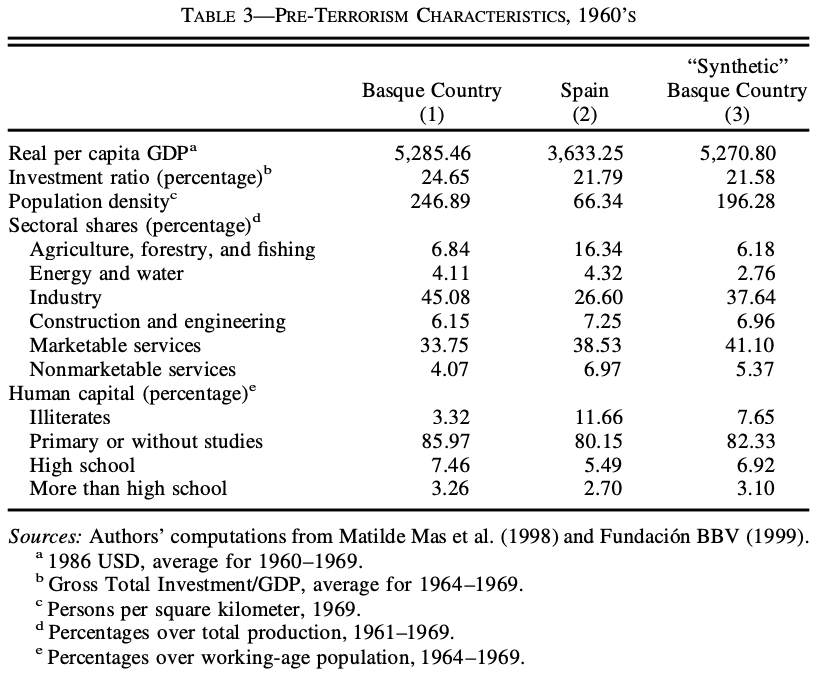
\includegraphics[width = .6\textwidth]{figures/balance panel all.png}
        \label{fig:balance_all}
    \end{figure}
\end{frame}

\begin{frame}{Methods}
    \begin{figure}
        \centering
        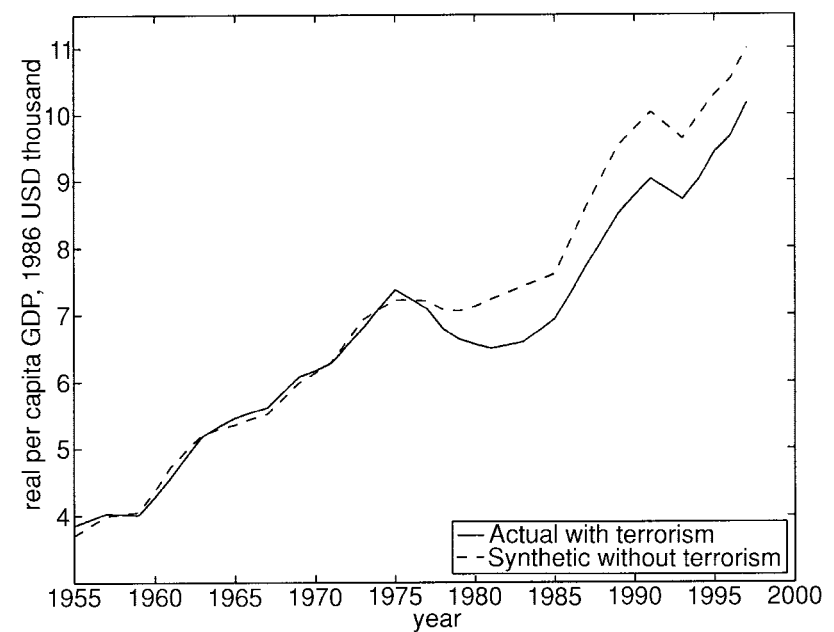
\includegraphics[width = .6\textwidth]{figures/ts.png}
        \label{fig:ts}
    \end{figure}
\end{frame}

\section{Estimating costs of Basque conflict}    

\begin{frame}{Estimating costs of Basque conflict}
    \begin{wideitemize}
        \item Now we simply compare the outcomes of the treatment and control groups after the treatment period. 
    \end{wideitemize}
\end{frame}

\begin{frame}{Estimating costs of Basque conflict}
    \begin{figure}
        \centering
        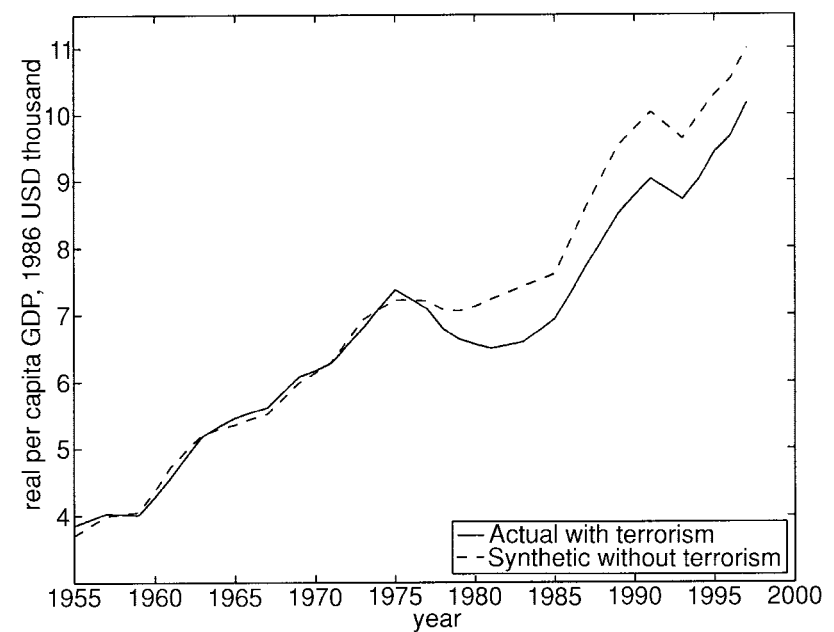
\includegraphics[width = .7\textwidth]{figures/ts.png}
        \label{fig:ts_1}
    \end{figure}
\end{frame}

\begin{frame}{Estimating costs of Basque conflict}
    \begin{figure}
        \centering
        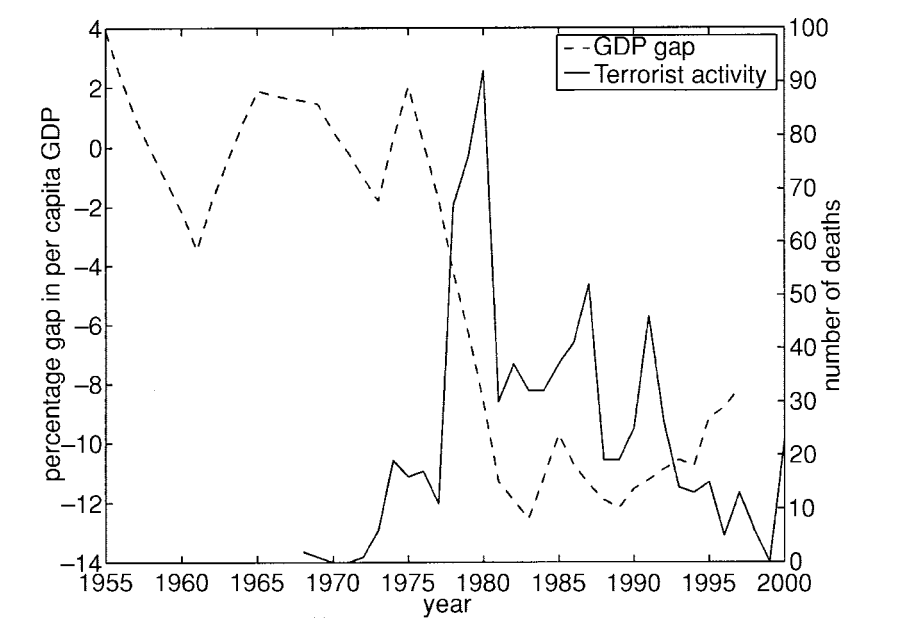
\includegraphics[width = .7\textwidth]{figures/ts1.png}
        \label{fig:ts_11}
    \end{figure}
\end{frame}

\begin{frame}{Estimating costs of Basque conflict}
    It is also interesting to note that Catalonia hosted the olympic games in 1992. \medskip 
    \begin{wideitemize}
        \item We expect this to increase per capita GDP relative to non-hosting regions.
        \item Hence we expect the gap between synthetic and real Basque region to be larger than estimated. 
    \end{wideitemize}

        \begin{figure}
    \centering
        
\includegraphics[width = .2\linewidth]{figures/barcelona_olympics.png}
        \label{fig:olympics}
    \end{figure}
    
\end{frame}

\begin{frame}{Estimating costs of Basque conflict}
    Takeaways from this exercise: \medskip 
    \begin{wideitemize}
        \item The actual Basque region grows below the control Basque region
        \item Larger deviations from control are associated with terrorist activity
        \item The magnitude of the effect is about 10\%
        \item We should check with "placebo" studies and other robustness checks
    \end{wideitemize}
\end{frame}

\section{Applications}

\begin{frame}{Applications - Overview}

    Synthetic control methods have found been applied widely
    in fields such as: \\ \medskip
    \begin{wideitemize}
        \item Economics: \cite{gautier_terrorism_2009} \cite{billmeier_assessing_2013}, \cite{cavallo_catastrophic_2013}
        \item Political Science: \cite{abadie_synthetic_2010}, \cite{abadie_comparative_2015}
        \item Health Policy: \cite{kreif_examination_2016} \cite{li_removing_2021}
        \item Criminology: \cite{saunders_synthetic_2015}
    \end{wideitemize}
    \medskip
    There is also a nice review article: \cite{abadie_using_2021} 
\end{frame}

\begin{frame}{Applications - Overview}

    \textcolor{lightgray}{Synthetic control methods have found been applied widely
    in fields such as:} \\ \medskip
    \begin{wideitemize}
        \item \textcolor{lightgray}{Economics: \cite{gautier_terrorism_2009} \cite{billmeier_assessing_2013}, \cite{cavallo_catastrophic_2013}}
        \item \textcolor{lightgray}{Political Science:}\textbf{ \cite{abadie_synthetic_2010},} \textcolor{lightgray}{\cite{abadie_comparative_2015}}
        \item \textcolor{lightgray}{Health Policy: \cite{kreif_examination_2016} \cite{li_removing_2021}}
        \item \textcolor{lightgray}{Criminology: \cite{saunders_synthetic_2015}}
    \end{wideitemize}
    \medskip
    \textcolor{lightgray}{There is also a nice review article: \cite{abadie_using_2021} }
\end{frame}

\begin{frame}{Applications: Abadie et al. (2010)}

    \begin{wideitemize}
        \item In 1988, California voters passed \textbf{1988 Proposition 99}
        \item The law included a 25-cent excise tax per carton of cigarettes
        \item What is an appropriate counterfactual? \pause \textbf{Construct a synthetic California} \pause 
    \end{wideitemize}
    \medskip \medskip \medskip \medskip
    \[\texttt{CA} = 0.164 (\texttt{CO}) + 0.069 (\texttt{CT}) + 0.199 (\texttt{MT}) + 0.234 (\texttt{NV}) + 0.334 (\texttt{UT})\]
\end{frame}

\begin{frame}{Applications: Abadie et al. (2010)}
    
    \begin{figure}
        \centering
        \begin{subfigure}{.45 \textwidth}
            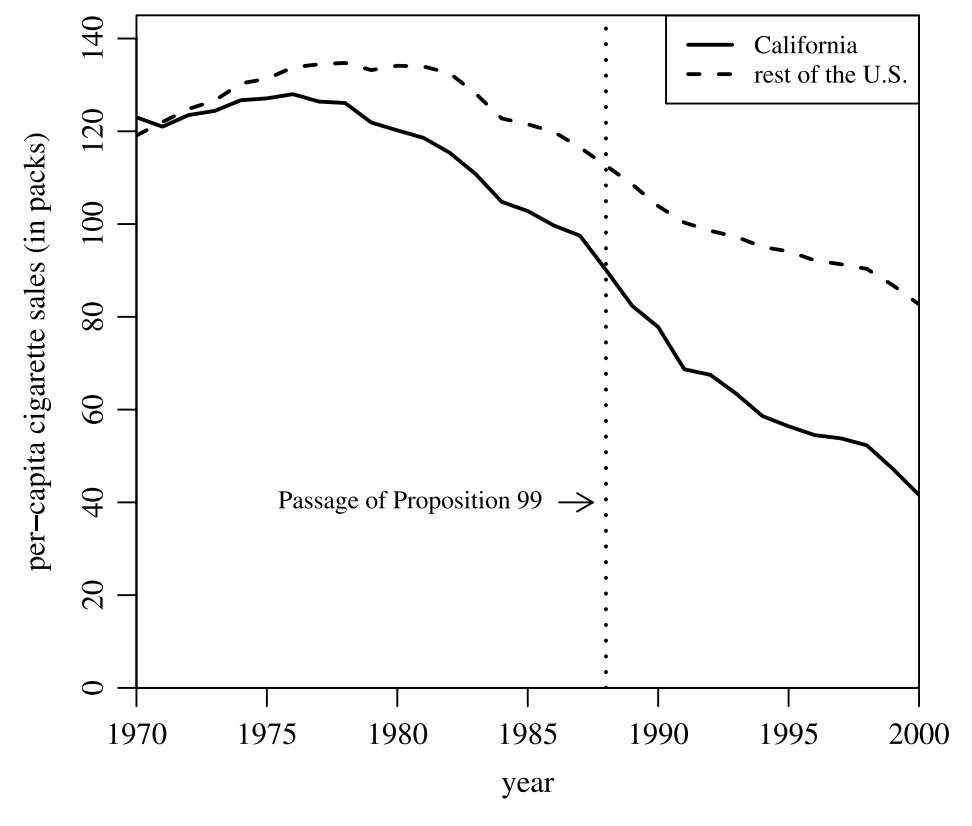
\includegraphics[width = \linewidth]{figures/ca_row.png}
        \end{subfigure} 
        \begin{subfigure}{.45 \textwidth}
            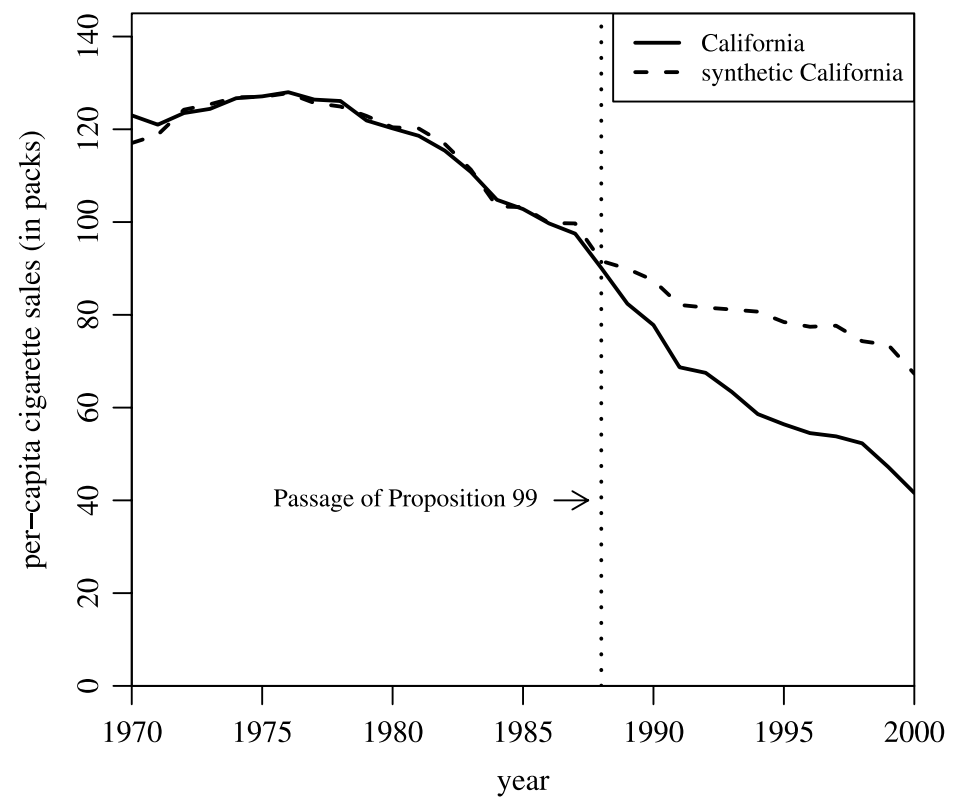
\includegraphics[width = \linewidth]{figures/ca_synthca.png}
        \end{subfigure}
    \end{figure}
    
    Headline: CA cigarette sales p.c. were \textbf{26 packs lower} because of Proposition 99. 
    
\end{frame}

\begin{frame}{Applications - Overview}

    \textcolor{lightgray}{Synthetic control methods have found been applied widely
    in fields such as:} \\ \medskip
    \begin{wideitemize}
        \item \textcolor{lightgray}{Economics: \cite{gautier_terrorism_2009} \cite{billmeier_assessing_2013}, \cite{cavallo_catastrophic_2013}}
        \item \textcolor{lightgray}{Political Science: \cite{abadie_synthetic_2010},} \textbf{\cite{abadie_comparative_2015}}
        \item \textcolor{lightgray}{Health Policy: \cite{kreif_examination_2016} \cite{li_removing_2021}}
        \item \textcolor{lightgray}{Criminology: \cite{saunders_synthetic_2015}}
    \end{wideitemize}
    \medskip
    \textcolor{lightgray}{There is also a nice review article: \cite{abadie_using_2021} }
\end{frame}

\begin{frame}{Applications: Abadie et al. (2015)}

    \begin{wideitemize}
        \item On November 9, 1989, the Berlin Wall fell
        \item West German GDP per capita was triple that of East Germany
        \item Question: What was the effect of integration on the West German economy? 
    \end{wideitemize}   

\end{frame}

\begin{frame}{Applications: Abadie et al. (2015)}
    \begin{figure}
    \centering
        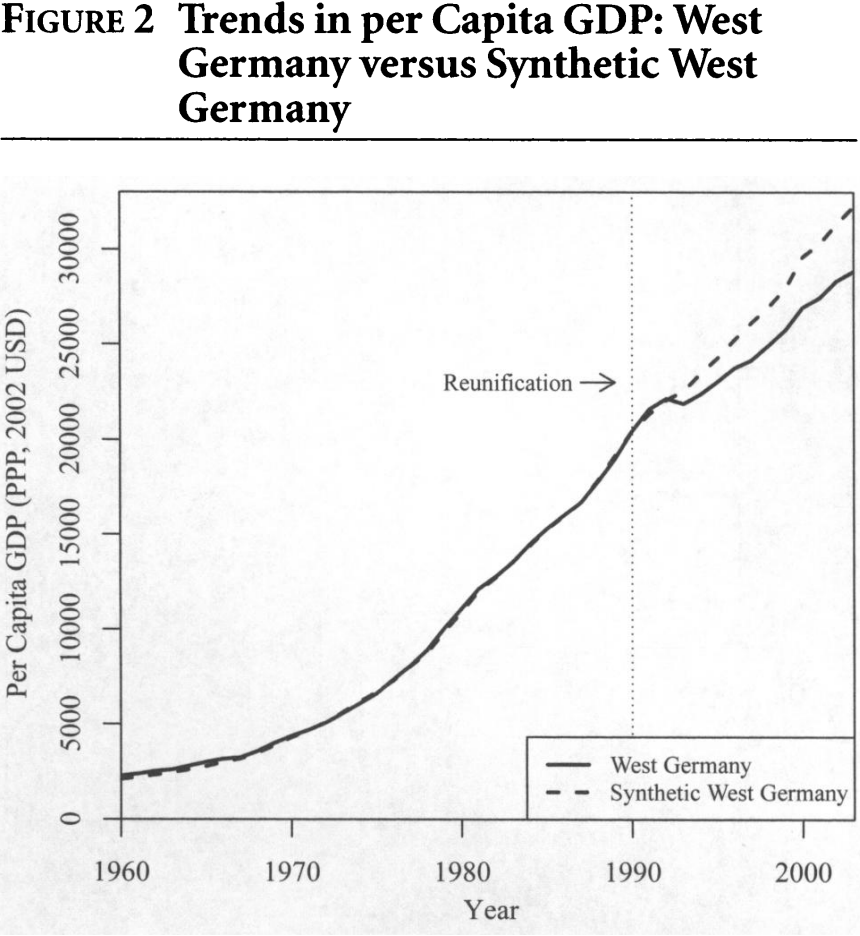
\includegraphics[width = .4\linewidth]{figures/adh2015.png}
        \label{fig:abadie2015}
    \end{figure}
    
    \small Headline: 2003 per capita GDP in synthetic W. Germany is 12\% higher than in reality
\end{frame}


\section{Software}

\begin{frame}{Active community building software}
    Focusing on R: 
    \medskip

    \begin{wideitemize}
        \item \textcolor{blue}{\texttt{\href{https://cran.r-project.org/web/packages/Synth/index.html}{synth}}} (Diamond, Hainmueller, originally 2007): classic implementation
            \begin{wideitemize} 
            \item includes data sets Basque data set from \cite{abadie_economic_2003} 
            \end{wideitemize}
        \item \textcolor{blue}{\texttt{\href{https://cran.r-project.org/web/packages/tidysynth/index.html}{tidysynth}}} (Dunford, 2021): a tidy implementation of sc conducive to piping 
        \item \textcolor{blue}{\texttt{\href{https://yiqingxu.org/packages/gsynth/}{gsynth}}} (Xu, Liu 2021): generalized synthetic control methods
        \item \textcolor{blue}{\texttt{\href{https://nppackages.github.io/scpi/}{scpi}}} (Cattaneo et al., October 2022): uncertainty quantification for synthetic control methods
    \end{wideitemize}
\end{frame}
   
% BIBLIOGRAPHY
\begin{frame}[allowframebreaks]{References}
\printbibliography
\end{frame}

\end{document}